\chapter{Progettazione e realizzazione}\label{capitolo:progettazione_realizzazione}
\markboth{Progettazione e realizzazione}{}
Questo capitolo è dedicato alla comprensione e descrizione delle fasi di progettazione e realizzazione di \visualnetkit{}. Si mostretà in maniera dettagliata la nuova struttura dei \plugin{} accennata nel precedente capitolo, e successivamente verrà mostrato il resto del sistema analizzando i singoli moduli che lo compongono.

\begin{figure}[!htb]
	\centering
	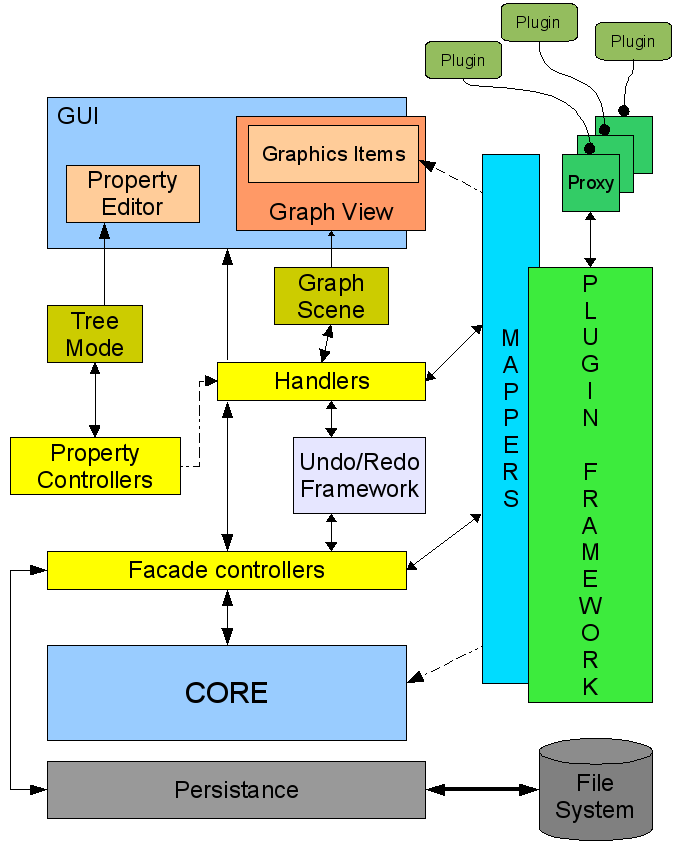
\includegraphics[width=8cm]{images/diagramma_componenti_vnetkit.png}
	\caption{Diagramma dei componenti di \visualnetkit{}}
	\label{figura:vn_componenti}
\end{figure}

In questa introduzione vogliamo subito dare al lettore un quadro generale (figura \ref{figura:vn_componenti}) della composizione architetturale nello stato attuale di \visualnetkit{}, in modo da rendere più facile la localizzazione degli elementi durante la loro trattazione.

\section{Architettura modulare basata su \plugin{}}
\subsection{Interazione tra sistema e \plugin{}}

\section{Elementi architetturali}

\subsection{L'interfaccia utente}


\subsection{Gli handlers}

\subsection{Property controllers}

\subsection{Undo Framework}

\subsection{Elementi del dominio}

\subsection{L'accesso al \fs{}}

\subsection{I mappers}

\section{La gestione avanzata delle properties}
\subsection{Properties di base}
\subsection{Properties dei \plugin{}}

\section{Strumenti di supporto allo sviluppo}
\subsection{Il framework \qt{}}
\subsection{Altri strumenti secondari}
